\documentclass{saco}
\begin{document}
\maketitle

\section{Introduction}
Rob the Robot has been programmed to map the subway networks of various cities automatically.
For each city, he has explored the subway network and recorded some information about his exploration, which will be used to create a map.
Unfortunately, due to a programming error, Rob has explored some of the subway networks more than once, and he does not know how many cities he has visited in total.

Given the recorded information for each subway network, you must help determine the number of different subway networks that Rob has explored.

\section{Task}
A subway network consists of a number of \emph{stations}, and a number of \emph{lines}, each of which connects two stations, such that there is exactly one way to travel between any two stations without traveling on the same line twice (in other words, there are no loops in the network).
Rob explores each subway network by starting at a random station, and then traveling along the lines to visit each other station, before returning to his starting position.
He does this in the least possible number of trips, so that he travels along each line exactly twice: once going away from his starting position, and then once returning towards it.
However, he does not attempt to visit the stations in any particular order.

When Rob travels along a line for the first time, he writes down a 0, and when he travels along it for the second time, he writes down a 1, hence obtaining a string of 0s and 1s describing the subway network.
Each city has a unique subway network, so it is impossible to obtain the same strings for two different cities, regardless of the station that Rob starts at.
However, it may be possible to obtain different strings for the same network.

He now has a collection of strings of 0s and 1s, each of the same length $V$, describing different subway networks; however, some of them may in fact describe the same subway network.
Your goal is to determine, given this information, the number of different subway networks that he has explored.

\section{Example}
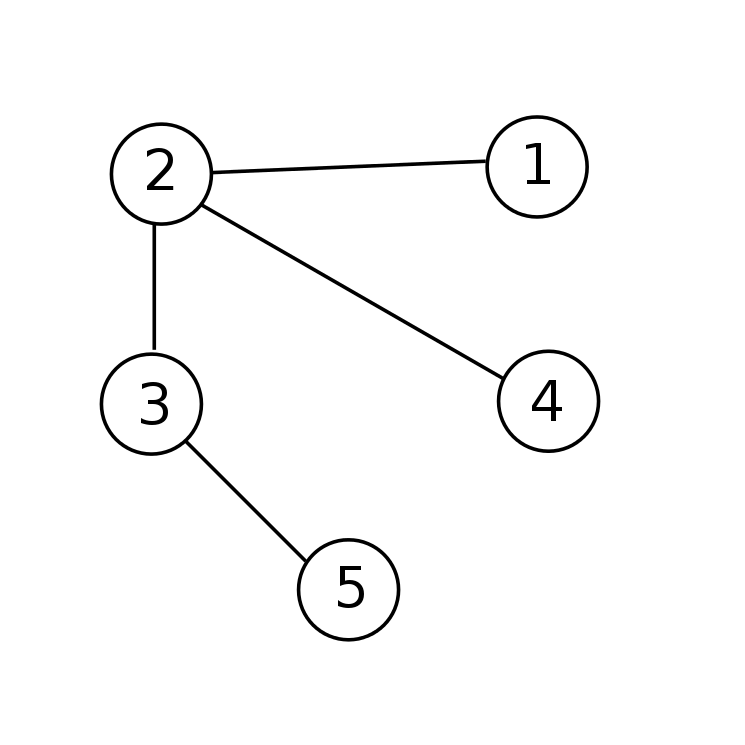
\includegraphics[height=5cm]{image/example.png}

In the above example, if Rob starts at station 4, and takes the route $4\rightarrow2\rightarrow1\rightarrow2\rightarrow3\rightarrow5\rightarrow3\rightarrow2\rightarrow4$, then he will obtain the string 00100111 describing the subway network.
He could also obtain the string 00011011 by starting at station 4, and taking the route $4\rightarrow2\rightarrow3\rightarrow5\rightarrow3\rightarrow2\rightarrow1\rightarrow2\rightarrow4$.
However, he could never obtain the string 00001111 no matter what station he starts at, or what route he takes.
This string then must correspond to a different subway network.

\inputformat
The first line of input will consist of an integer $N$, the number of records Rob has.
The following $N$ lines will each consist of a string of 0s and 1s. All strings will be of the same length $V$.
\sampleinput

\outputformat
The output should contain a single integer $M$, the number of distinct subway networks that Rob has explored.
\sampleoutput

\section{Constraints}
\begin{itemize}
\item $1 \leq N \leq 1000$
\item $1 \leq V \leq 30$
\end{itemize}

Additionally, in 30\% of the test cases:
\begin{itemize}
\item $1 \leq N \leq 50$
\item Whenever Rob visits the same city more than once, he starts at the same station in each case.
\end{itemize}

Additionally, in 60\% of the test cases:
\begin{itemize}
\item Whenever Rob visits the same city more than once, he starts at the same station in each case.
\end{itemize}

\timelimit

\feedback

\section{Scoring}
A correct solution will score 100\% while an incorrect solution will score 0\%.

\end{document}
